\begin{frame}
    \begin{center}
        {\large Laplace Mean-Field Approximation}
    \end{center}        
\end{frame}

\begin{frame}[t]
    \frametitle{Noisy observation}
    Usually, observations $\dymytn{} = [\mrange{\dymyktn{1}{}}{\dymyktn{K}{}}]^\top \in \R^{K}$ are contaminated by noises $\dymepsilontn{} = [\mrange{\epsilon_1(t_{})}{\epsilon_K(t_{})}] \in \R^{K}$ such that
    \begin{align}
        \dymytn{} = \dymxtn{} + \dymepsilontn{}        
    \end{align}
    
    \vspace{\baselineskip}
    For a sequence of observations, we denote
    \begin{align}
        \dymY & = [\mrange{\dymytn{1}}{\dymytn{N}}] \in \R^{K \times N}
        \nonumber
        \\
        \dymX & = [\mrange{\dymxtn{1}}{\dymxtn{N}}] \in \R^{K \times N}
        \nonumber
        \\
        \dymE & = [\mrange{\dymepsilontn{1}}{\dymepsilontn{N}}] \in \R^{K \times N}
        \nonumber
    \end{align}
\end{frame}

\begin{frame}[t]
    \frametitle{Noisy observation}
    Assuming \emph{independent and identically distributed (i.i.d.)} state-specific, additive Gaussian noise $\dymepsilon{(t)} \sim \mathcal{N}(\mvector{0}, \mvector{D})$ with $\mvector{D} = diag(\mrange{\dymsigmak{1}^2}{\dymsigmak{K}^2}) \in R^{K \times K}$, then
    \begin{align}        
        p(\dymY\vert\dymX,\dymsigma) 
        & = \prod_k{
            p(\dymyk{k}\vert\dymxk{k},\dymsigmak{k})
        }
        \nonumber
        \\
        & = \prod_k{
            \mathcal{N}(\dymyk{k}\vert\dymxk{k}, \dymsigmak{k}^2\mI)
        }
        \label{eq-ode-noise-model} 
    \end{align}
    where 
    \begin{itemize}    	
    	\item[] $\dymyk{k} = [\mrange{\dymyktn{k}{1}}{\dymyktn{k}{N}}]^\top \in \R^N$ are the observations for the $k$-th state over time.
        \item[] $\dymxk{k} = [\mrange{\dymxktn{k}{1}}{\dymxktn{k}{N}}]^\top \in \R^N$ are the values of the $k$-th state over time.
    \end{itemize}
\end{frame}

\begin{frame}[t]
    \frametitle{State prior}
    Introducing state-specific, independent Gaussian process priors on each $\dymxk{k}$ for $k = \mrange{1}{K}$, then
    \begin{align}
        p(\dymX\vert\dymphi) 
        & = 
        \prod_k{
            p(\dymxk{k}\vert\dymphik{k})
        }
        \nonumber
        \\
        & = 
        \prod_k{
            \mathcal{N}(
            \dymxk{k}\vert\mvector{0}, \dymCphik{k})
        }
        \label{eq-gmgp-x-prior}
    \end{align}
    where $\dymCphik{k}$ is the covariance matrix induced by the kernel function $\dymkernel{k}$ with hyperparemeter $\dymphik{k}$.
\end{frame}

\begin{frame}[t]
    \frametitle{State posterior}
    Using \emph{Bayes' theorem}, the posterior on $\dymX$ is obtained as
    \begin{align}
        p(\dymX\vert\dymY,\dymphi,\dymsigma) 
        & = 
        \frac{
            p(\dymX\vert\dymphi)p(\dymY\vert\dymX,\dymsigma)}{
            \int{
                p(\dymX\vert\dymphi)p(\dymY\vert\dymX,\dymsigma)d{\dymX}}
        }
        \nonumber
        \\
        & = 
        \prod_k{
            p(\dymxk{k}\vert\dymyk{k},\dymphik{k},\dymsigmak{k})
        }
        \nonumber
        \\
        & = 
        \prod_k{
            \mathcal{N}(
            \dymxk{k}\vert\dymmuk{k}, \dymSigmak{k})
        }
        \label{eq-gmgp-x-posterior}
    \end{align}
    where
    \begin{align}
        \dymmuk{k} &= \dymCphik{k}(\dymCphik{k} + \dymsigmak{k}^2\mI)^{-1}\dymyk{k}
        \nonumber
        \\        
        \dymSigmak{k} &= \dymsigmak{k}^2\dymCphik{k}(\dymCphik{k} + \dymsigmak{k}^2\mI)^{-1}
        \nonumber
    \end{align}    
\end{frame}

\begin{frame}[t]
    \frametitle{Gaussian process response model}
    Because Gaussian process is closed under differentiation, the joint distribution of $\dymxk{k}$ and $\dymdxk{k}$, for $k = \mrange{1}{K}$, within a finite amount of time points is also Gaussian:
    \begin{align}
        \begin{bmatrix}
            \dymxk{k}
            \\ 
            \dymdxk{k}
        \end{bmatrix}
        & \sim 
        \mathcal{N}(
            \begin{bmatrix}
                \mvector{0} 
               \\ 
                \mvector{0}
            \end{bmatrix}
            ,\ 
            \begin{bmatrix}
                \dymCphik{k} & \dymCdphik{k}
                \\ 
                \dymdCphik{k} & \dymdCdphik{k}
            \end{bmatrix}
        )
    \end{align}
    where
    \begin{columns}
        \begin{column}{0.15\textwidth}            
        \end{column}
        \begin{column}{0.35\textwidth}
            \begin{align}
                \dymCphikij{k} 
                & = \dymkernel{k}(\dymtn{i}, \dymtn{j})
                \nonumber    
                \\
                \dymdCphikij{k} 
                & = \frac{\partial\dymkernel{k}(\dymtn{i}, \dymtn{j})}
                {\partial\dymtn{i}}
                \nonumber            
            \end{align}
        \end{column}
        \begin{column}{0.35\textwidth}    
            \begin{align}
                \dymCdphikij{k} 
                & = \frac{\partial\dymkernel{k}(\dymtn{i}, \dymtn{j})}
                {\partial\dymtn{j}}
                \nonumber
                \\
                \dymdCdphikij{k} 
                & = \frac{\partial^2\dymkernel{k}(\dymtn{i}, \dymtn{j})}
                {\partial\dymtn{i}\partial\dymtn{j}}
                \nonumber
            \end{align}
        \end{column}
        \begin{column}{0.15\textwidth}            
        \end{column}
    \end{columns}     
\end{frame}

\begin{frame}[t]
    \frametitle{Gaussian process response model}
    The conditional distribution over $\dymdX$ is given by
    \begin{align}
        p(\dymdX\vert\dymX,\dymphi) 
        & = 
        \prod_k{
            p(\dymdxk{k}\vert\dymxk{k},\dymphik{k})
        }
        \nonumber
        \\
        & = 
        \prod_k{
            \mathcal{N}(\dymdxk{k}\vert\dymmk{k}, \dymAk{k})
        }        
        \label{eq-gmgp-dx-posterior}
    \end{align}            
    where
    \begin{align}
        \dymmk{k} & = \dymdCphik{k}\dyminvCphik{k}\dymxk{k}
        \nonumber
        \\
        \dymAk{k} & = \dymdCdphik{k} - \dymdCphik{k}\dyminvCphik{k}\dymCdphik{k}
        \nonumber
    \end{align}    
\end{frame}

\begin{frame}[t]
    \frametitle{ODE response model}
    Assuming state-specific, additive Gaussian errors between $\dymdx$ and the response from $\dymf$, we have
    \begin{align}
        p(\dymdX\vert\dymX,\dymtheta,\dymgamma) 
        & = 
        \prod_k{
            p(\dymdxk{k}\vert\dymX,\dymtheta,\dymgammak{k})
        }
        \nonumber
        \\
        & = 
        \prod_k{
            \mathcal{N}(\dymdxk{k}\vert\dymfkX{k},\dymgammak{k}\mI)
        }
        \label{eq-gmgp-dx-ode-response}
    \end{align}
    where 
    \begin{itemize}
    	\item[] $\dymdxk{k} = [\mrange{\dymdxktn{k}{1}}{\dymdxktn{k}{N}}] \in \R^N$ are the derivatives for the $k$-th state over time.
    	\item[] $\dymgamma = [\mrange{\dymgammak{1}}
    {\dymgammak{K}}]^T \in \R^K$ contains the error variances.
    \end{itemize}
\end{frame}

\begin{frame}[t]
    \frametitle{Product of experts}
    \begin{columns}
        \begin{column}{0.65\textwidth}            
            The \emph{product of experts} technique combines \refequationp{\ref{eq-gmgp-dx-posterior}} and \refequationp{\ref{eq-gmgp-dx-ode-response}} to obtain
            \begin{align}
                p(\dymdX\vert\dymX,\dymphi,\dymtheta,\dymgamma)
                \propto p(\dymdX\vert\dymX,\dymphi) p(\dymdX\vert\dymX,\dymtheta,\dymgamma) 
                \label{eq-gmgp-poe}
            \end{align}
            which attains high densities where both $p(\dymdX\vert\dymX,\dymphi)$ and $p(\dymdX\vert\dymX,\dymtheta,\dymgamma)$ have strong support. 
        \end{column}
        \begin{column}{0.35\textwidth}       
            \begin{figure}
                \centering
                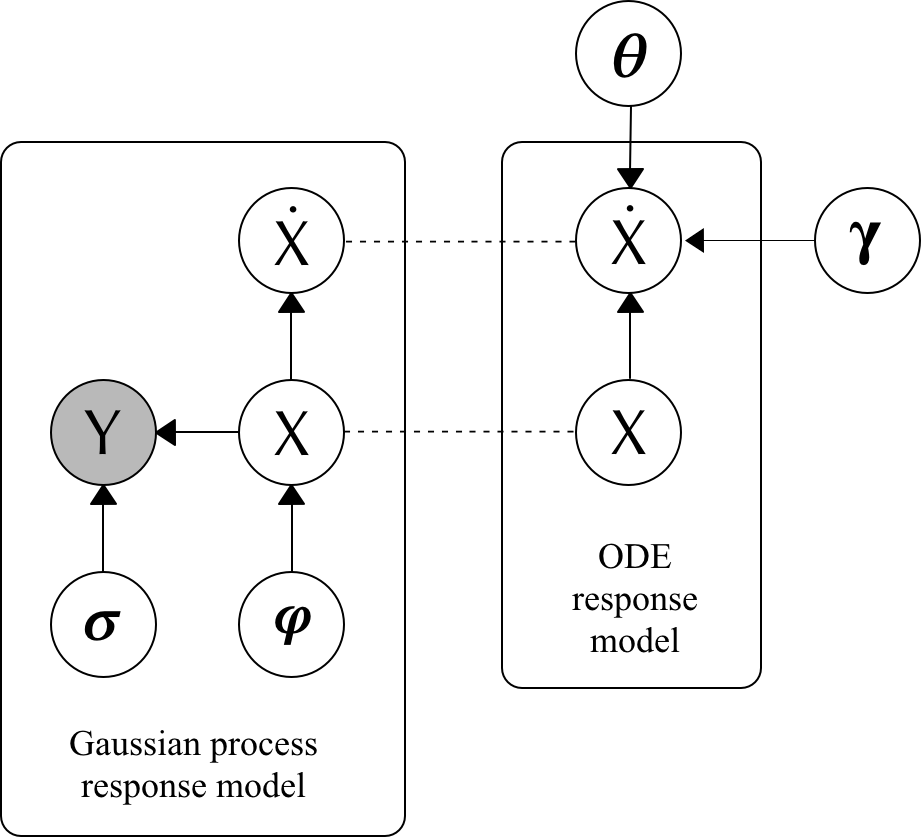
\includegraphics[width=1\textwidth]{graphics/gradient-matching-model}                    
            \end{figure} 
        \end{column}
    \end{columns}
\end{frame}

\begin{frame}[t]
    \frametitle{Joint posterior}
    The joint posterior $p(\dymX,\dymtheta\vert\dymY,\dymphi,\dymsigma,\dymgamma)$ is obtained by
    \begin{align}
        p(\dymX,\dymtheta\vert\dymY,\dymphi,\dymsigma,\dymgamma)         
        & =      
        \int{
            p(\dymtheta)p(\dymX\vert\dymY,\dymphi,\dymsigma) p(\dymdX\vert\dymX,\dymtheta,\dymphi,\dymgamma) d\dymdX
        }
        \nonumber
        \\
        & \propto
        p(\dymtheta) \prod_k{[
            \mathcal{N}(\dymxk{k}\vert\dymmuk{k}, \dymSigmak{k}) 
            \mathcal{N}(\dymfkX{k}\vert\dymmk{k},\dyminvLambdak{k})]}    
        \label{eq-vgmgp-posterior-joint}
    \end{align}
    where
    \begin{align}
        \dyminvLambdak{k} = \dymAk{k} + \dymgammak{k}\mvector{I} 
        \nonumber       
    \end{align}
    
    \vspace{\baselineskip}
	The ``best'' parameters $\dymtheta^*$ could be estimated using \emph{Maximum a posteriori (MAP)} to yield
    \begin{align}
        \dymtheta^*
        & = 
        \argmax_{\dymtheta}
            \int{p(\dymX,\dymtheta\vert\dymY,\dymphi,\dymsigma,\dymgamma)d\dymX}
        \nonumber
        \\
        & = 
        \argmax_{\dymtheta}
            p(\dymtheta\vert\dymY,\dymphi,\dymsigma,\dymgamma)        
        \label{eq-vgmgp-theta-posterior}
    \end{align}
    which is intractable due to strong non-linear couplings of the states inside the ODEs.    
\end{frame}
